moThe Higgs boson mass dependent signal selections are described in Section~\ref{sec:signal_selection}. 
In this section we summarise the results obtained all jet final states. 
Tables~\ref{tab:yield_mt_shapebased} shows the signal and 
equivalent data yields and background expectations in ee and $\mu\mu$ final states respectively. 
Figure~\ref{fig:histo_mt_250_5fb}-\ref{fig:histo_mt_600_5fb} show the $M_T$ distribution 
after the higgs mass dependent selections, for the mass hypothesis between 250 and 600 $\GeV$, 
corresponding to \intlumi. In these figures the background normalizations are scaled by 
each individual data-to-mc scale factors to account for the data and MC difference in 
background estimation described in section~\ref{sec:backgrounds}, 
lepton efficiency and the pileup reweighting. 

We consider the following uncertainties due to the shape variations, 
%%%%%%%%%%%%%%%%%%%%%%%%%%%%%
\begin{itemize}
\item {Statistic uncertainties in the template}
\item {QCD scale variations to the Higgs process}
\item {Top shape variations}
\item {WW shape variations}
\item {WZ shape variations}
\item {ZZ shape variations}.
\end{itemize}
%%%%%%%%%%%%%%%%%%%%%%%%%%%%%
The effects due to the lepton efficiency and scale variations are neglible and we assign only 
the normalization uncertainties. 
To understand the effects of the individual source of the uncertainties, 
we also compare the results by adding each source progressively, shown in Table~\ref{tab:mva_mtshape_detail}. 
Among all the shape systematics, the statistical uncertainty on the template is the leading effect. 
The details are documented in Ref.~\cite{shapeananote}. 

The expected cross section ratio limits as a function of the Higgs mass, together with the 1/2-$\sigma$ uncertainty 
bands are shown in Table~\ref{tab:limits_mtshape_5fb} and Figure~\ref{fig:limits_5fb}. 
The observed exclusion region for the Standard Model Higgs in [275,455]~\GeV{} at 95\%C.L., 
compared to the expected exclusion region as obic Higgs in [290,490]~\GeV{} at 95\%C.L.
Compared to the cut-based analysis, the shape analysis based on the $M_T$ variable improves the search sensitivity 
by upto $10\%$ considering all the shape variation systematics. 



%%%%%%%%%%%%%%%%%%%%%%%%%
\begin{table}[!ht]
{\small
 \begin{center}
 \begin{tabular}{l | c c | c c c c c c  | c}
 \hline\hline
 $mH$ & qqH & ggH & ZZ & ggZZ & WZ & WW/Top & Zjets & $\sum$Bkg & Data \\
 \hline
\multicolumn{10}{c} {ee} \\ 
\hline
250 & $0.8\pm0.1$ & $7.6\pm1.1$ & $15.4\pm1.6$ & $1.4\pm0.3$ & $11.0\pm1.4$ & $30.1\pm3.7$ & $6.0\pm6.0$ & $64.0\pm7.4$ & 60 \\
300 & $1.0\pm0.1$ & $9.1\pm1.4$ & $12.9\pm1.4$ & $1.1\pm0.3$ & $7.8\pm1.0$ & $17.0\pm2.8$ & $4.4\pm4.4$ & $43.2\pm5.5$ & 32 \\
350 & $1.0\pm0.1$ & $10.4\pm1.7$ & $14.9\pm1.6$ & $1.3\pm0.3$ & $8.7\pm1.1$ & $17.0\pm2.8$ & $5.0\pm5.0$ & $46.8\pm6.0$ & 35 \\
400 & $0.7\pm0.1$ & $8.8\pm1.5$ & $15.9\pm1.7$ & $1.4\pm0.3$ & $9.1\pm1.2$ & $17.0\pm2.8$ & $5.2\pm5.2$ & $48.5\pm6.2$ & 39 \\
500 & $0.4\pm0.1$ & $4.0\pm1.0$ & $17.0\pm1.8$ & $1.5\pm0.3$ & $9.4\pm1.2$ & $17.0\pm2.8$ & $5.4\pm5.4$ & $50.3\pm6.5$ & 39 \\
600 & $0.3\pm0.1$ & $1.7\pm0.6$ & $17.3\pm1.8$ & $1.5\pm0.3$ & $9.5\pm1.2$ & $17.0\pm2.8$ & $5.4\pm5.4$ & $50.8\pm6.5$ & 39 \\
\hline
\multicolumn{10}{c} {$\mu\mu$} \\ 
\hline
250 & $1.1\pm0.1$ & $10.7\pm1.5$ & $23.0\pm2.2$ & $2.1\pm0.5$ & $16.1\pm1.9$ & $37.5\pm4.5$ & $9.6\pm9.6$ & $88.4\pm11.1$ & 85 \\
300 & $1.4\pm0.1$ & $12.9\pm1.9$ & $18.8\pm1.8$ & $1.7\pm0.4$ & $11.2\pm1.3$ & $21.2\pm3.4$ & $7.0\pm7.0$ & $59.9\pm8.2$ & 60 \\
350 & $1.3\pm0.1$ & $14.8\pm2.3$ & $21.5\pm2.1$ & $1.9\pm0.4$ & $12.5\pm1.5$ & $21.2\pm3.4$ & $7.9\pm7.9$ & $65.0\pm9.0$ & 62 \\
400 & $1.0\pm0.1$ & $12.6\pm2.2$ & $23.1\pm2.3$ & $2.0\pm0.4$ & $13.1\pm1.5$ & $21.2\pm3.4$ & $8.2\pm8.2$ & $67.6\pm9.3$ & 65 \\
500 & $0.6\pm0.1$ & $5.5\pm1.3$ & $24.9\pm2.4$ & $2.2\pm0.5$ & $13.5\pm1.6$ & $21.2\pm3.4$ & $8.5\pm8.5$ & $70.2\pm9.6$ & 70 \\
600 & $0.3\pm0.1$ & $2.3\pm0.8$ & $25.3\pm2.5$ & $2.2\pm0.5$ & $13.6\pm1.6$ & $21.2\pm3.4$ & $8.6\pm8.6$ & $70.8\pm9.7$ & 70 \\
\hline\hline
\end{tabular}
\end{center}
}
\caption{Expected number of signal and background events for an 
  integrated luminosity of \intlumi after applying the higgs selections in the shape-based analysis in the ee final state. 
  Both statistical and systematic uncertainties are included. }
\label{tab:yield_mt_shapebased}
\end{table}

\begin{table}
\begin{center}
{\normalsize
\begin{tabular}{|l|c|c|c|c|c|c|}
\hline
      &  \multicolumn{3}{c|}{ without shape uncertainty} &\multicolumn{3}{c|}{ with shape uncertainty} \\
\hline
Mass  &  Median      &     68\% C.L. band &  95\% C.L. band &  Median	   &	 68\% C.L. band &  95\% C.L. band\\
      &  Expected    &                    &                 &  Expected    &			&		 \\
\hline
250 & 1.40 & [1.01, 1.94] & [0.76, 2.58] & 1.48 & [1.06, 2.05] & [0.80, 2.72] \\
300 & 0.92 & [0.66, 1.28] & [0.50, 1.69] & 0.93 & [0.67, 1.29] & [0.51, 1.72] \\
350 & 0.62 & [0.45, 0.86] & [0.34, 1.15] & 0.63 & [0.45, 0.87] & [0.34, 1.16] \\
400 & 0.63 & [0.45, 0.87] & [0.34, 1.16] & 0.63 & [0.46, 0.88] & [0.34, 1.17] \\
500 & 1.06 & [0.76, 1.47] & [0.57, 1.95] & 1.08 & [0.78, 1.50] & [0.58, 1.99] \\
600 & 2.20 & [1.59, 3.06] & [1.19, 4.06] & 2.23 & [1.61, 3.10] & [1.21, 4.12] \\
\hline
\end{tabular}
}
\end{center}
\caption{The median expected cross section ratio limits as a function 
of the Higgs mass, together with the 1/2-$\sigma$ uncertainty bands obtained in the shape analysis based on $M_T$, 
corresponding to an integrated luminosity of \intlumi}
\label{tab:limits_mtshape_5fb}
\end{table}

%%%%%%%%%%%%%%%%%%%%%%
\begin{figure}[!ht]
\begin{center}
   \subfigure[]{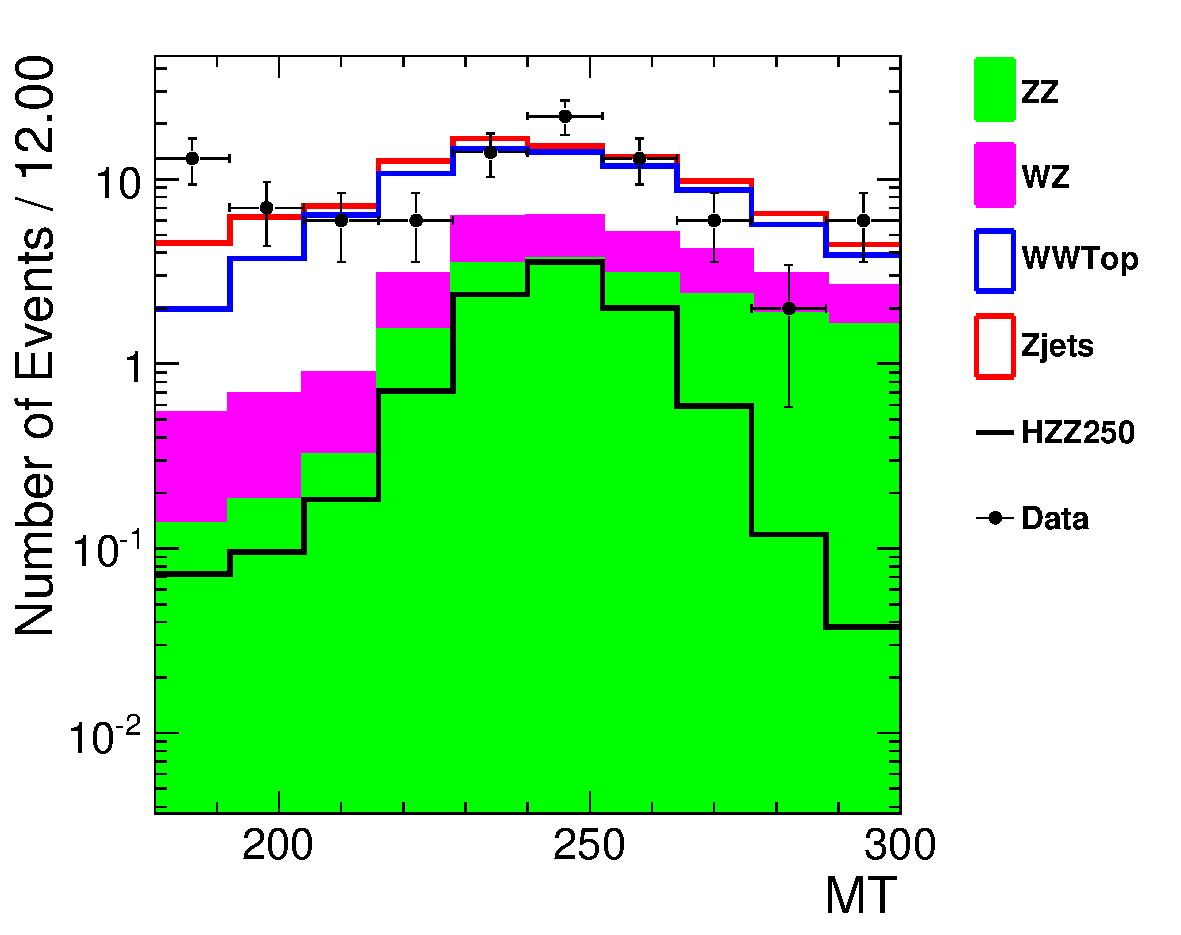
\includegraphics[width=0.4\textwidth,angle=0]{figures/MT_mH250_ee_stack_log.pdf}} 
   \subfigure[]{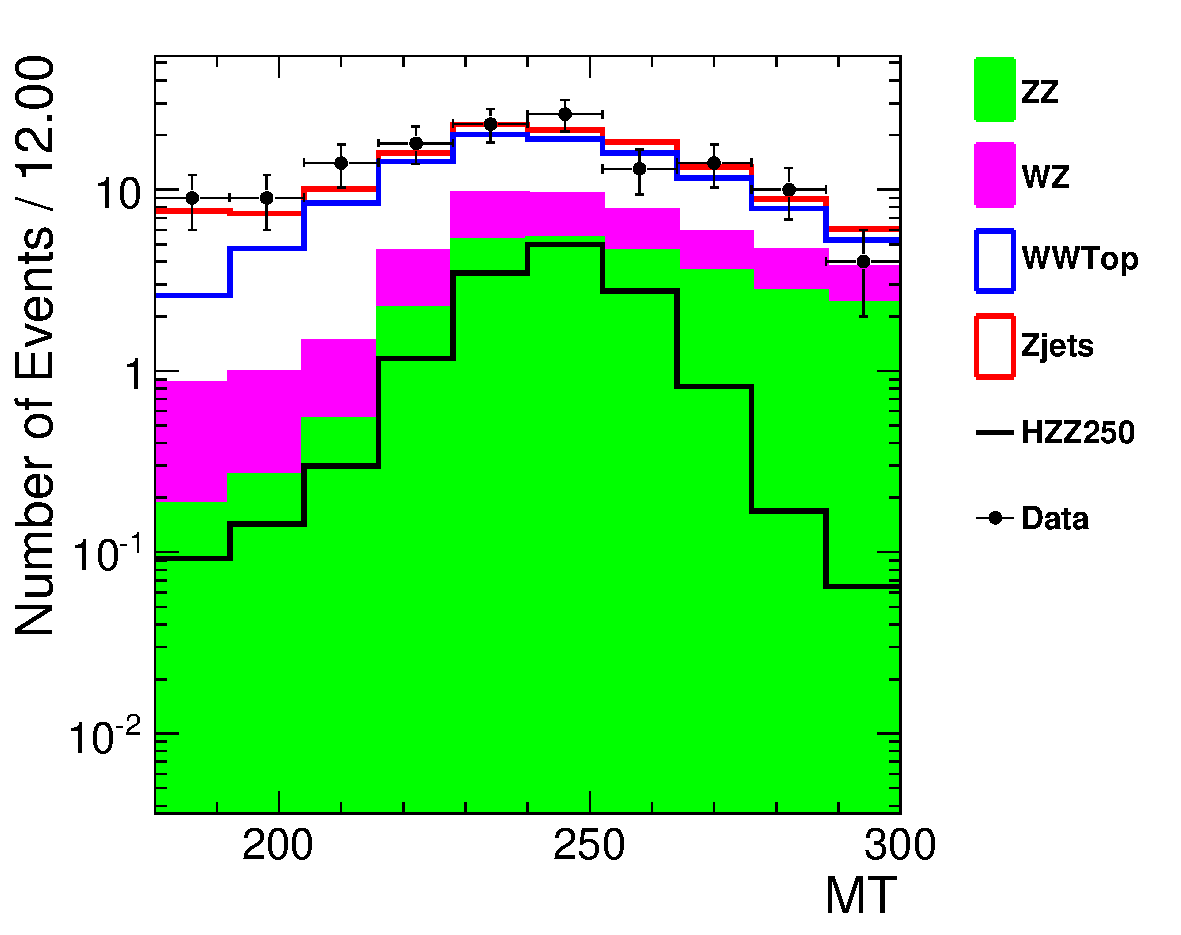
\includegraphics[width=0.4\textwidth,angle=0]{figures/MT_mH250_mm_stack_log.pdf}} \\ 
   \caption{The $M_T$ distribution for Higgs signal and background events 
for \mHi=250 $\GeVcc$ in ee (a) and $\mu\mu$ final state (b) after the higgs dependent selections. 
The distributions are normalized to \intlumi with the background scaled by the data-to-mc ratios derived from data.}
   \label{fig:histo_mt_250_5fb}
\end{center}
%\end{figure}

%\begin{figure}[!ht]
\begin{center}
   \subfigure[]{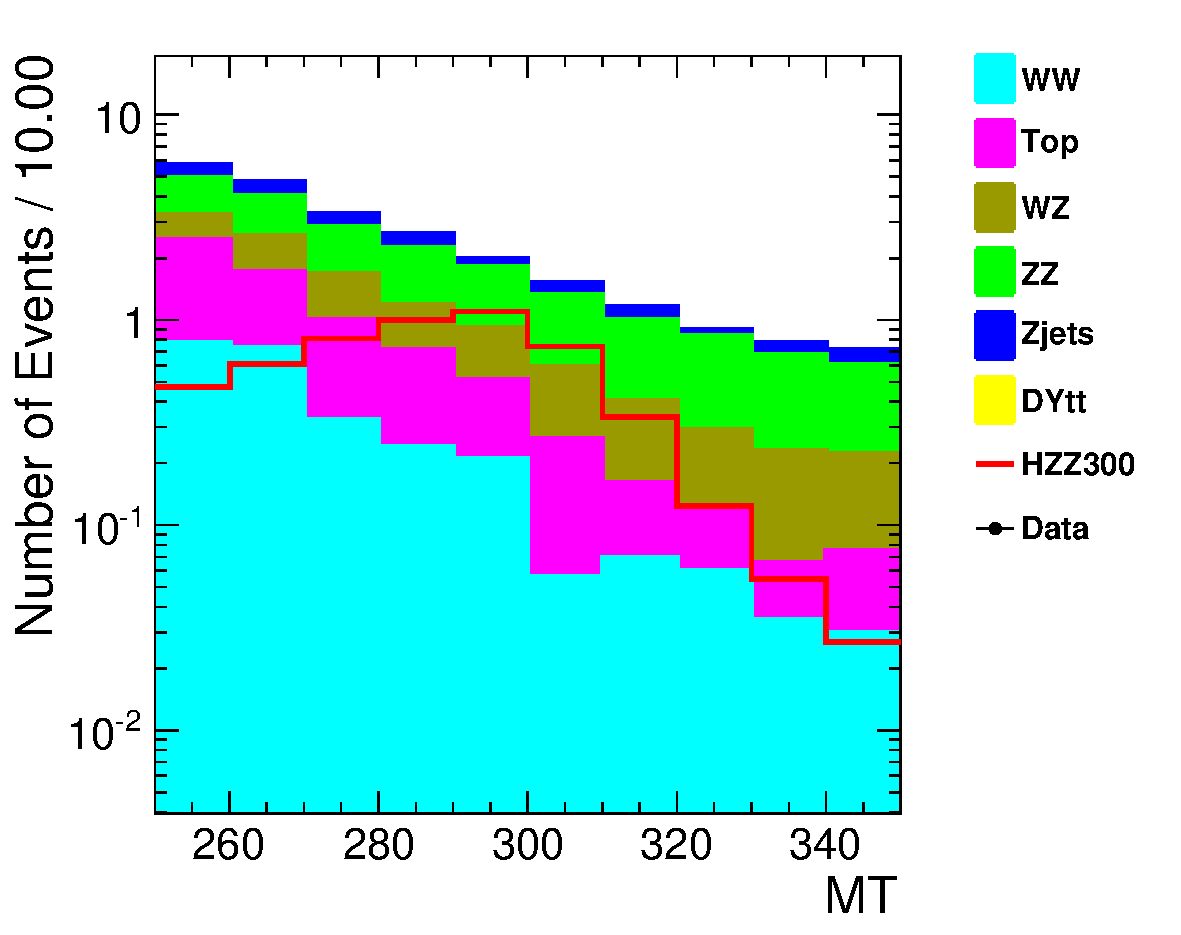
\includegraphics[width=0.4\textwidth,angle=0]{figures/MT_mH300_ee_stack_log.pdf}} 
   \subfigure[]{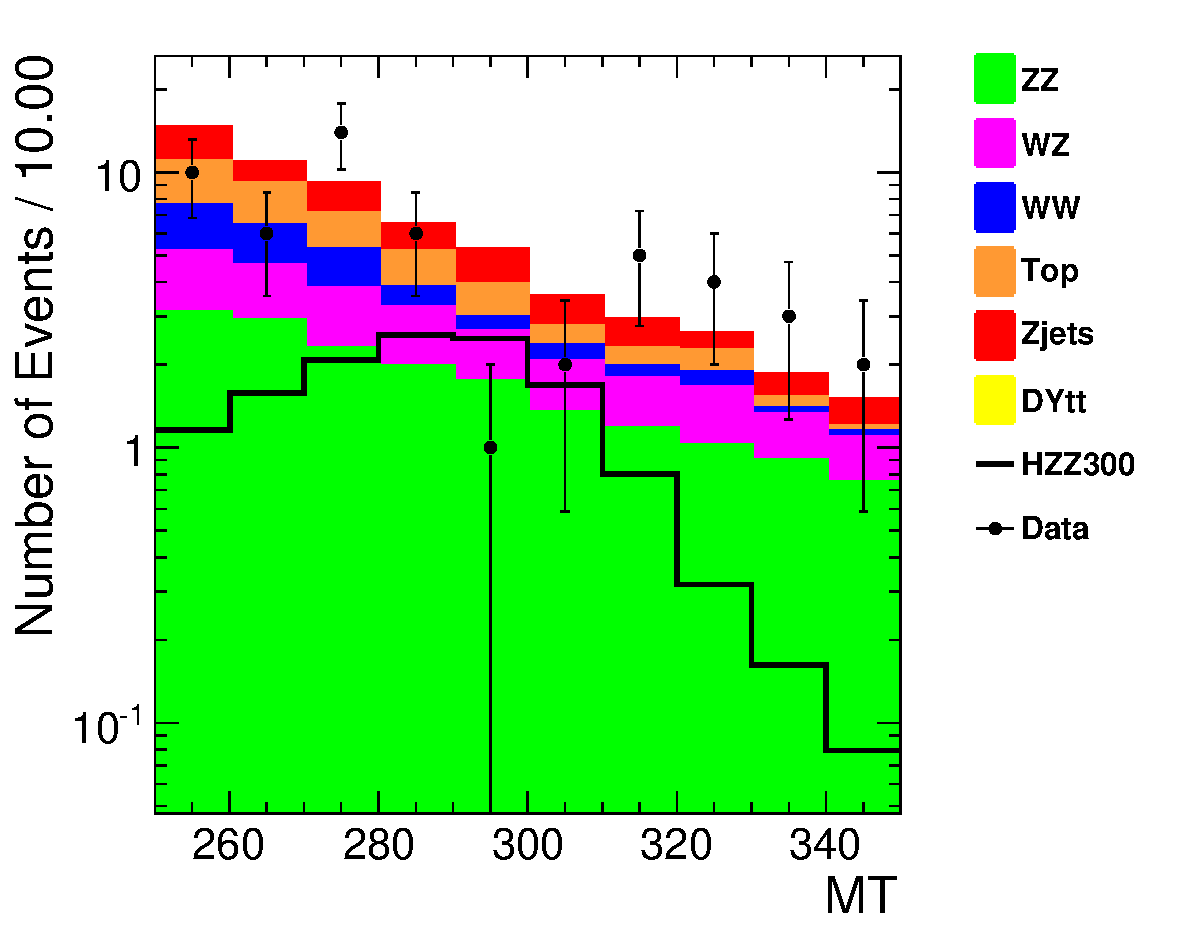
\includegraphics[width=0.4\textwidth,angle=0]{figures/MT_mH300_mm_stack_log.pdf}} \\ 
   \caption{The $M_T$ distribution for Higgs signal and background events 
for \mHi=300 $\GeVcc$ in ee (a) and $\mu\mu$ final state (b) after the higgs dependent selections. 
The distributions are normalized to \intlumi with the background scaled by the data-to-mc ratios derived from data.}
   \label{fig:histo_mt_300_5fb}
\end{center}
%\end{figure}

%\begin{figure}[!ht]
\begin{center}
   \subfigure[]{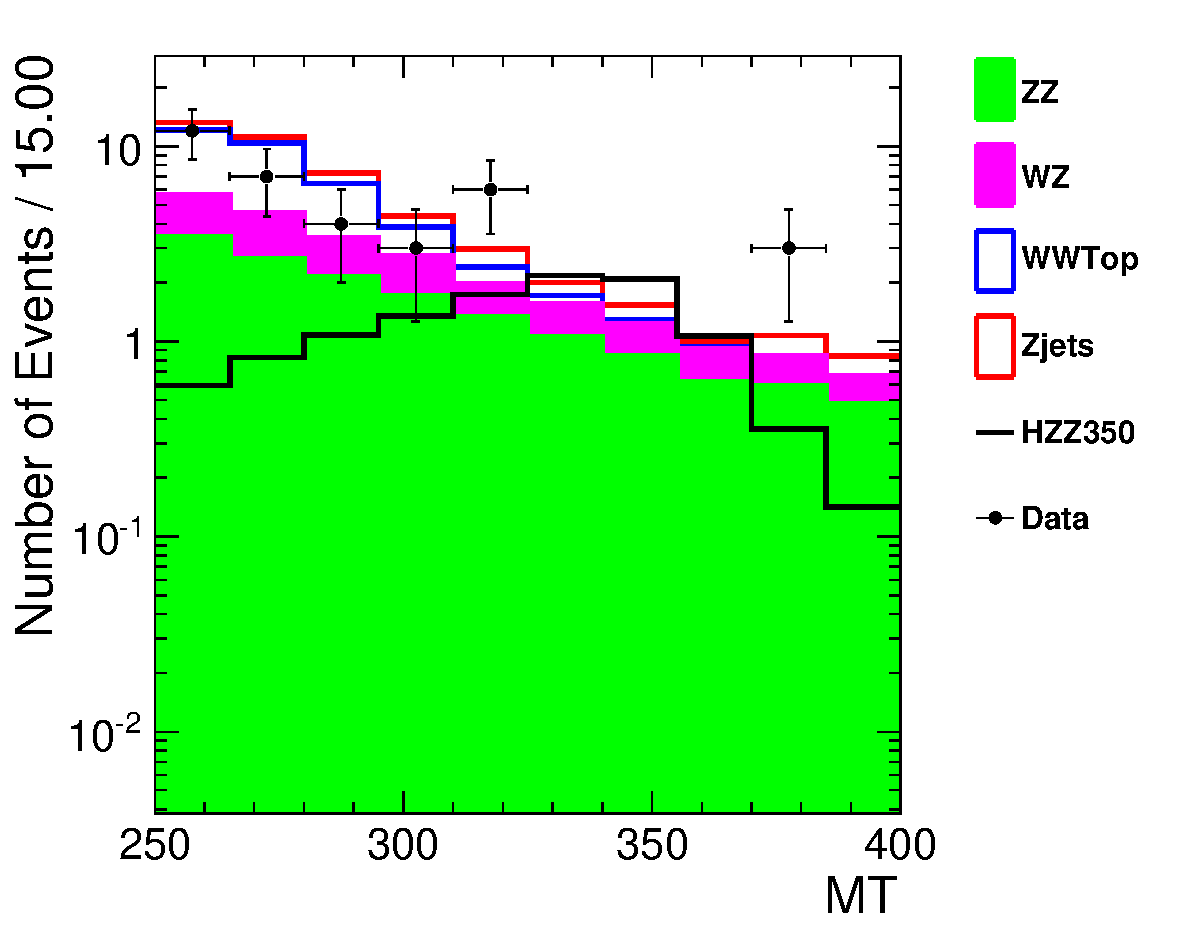
\includegraphics[width=0.4\textwidth,angle=0]{figures/MT_mH350_ee_stack_log.pdf}} 
   \subfigure[]{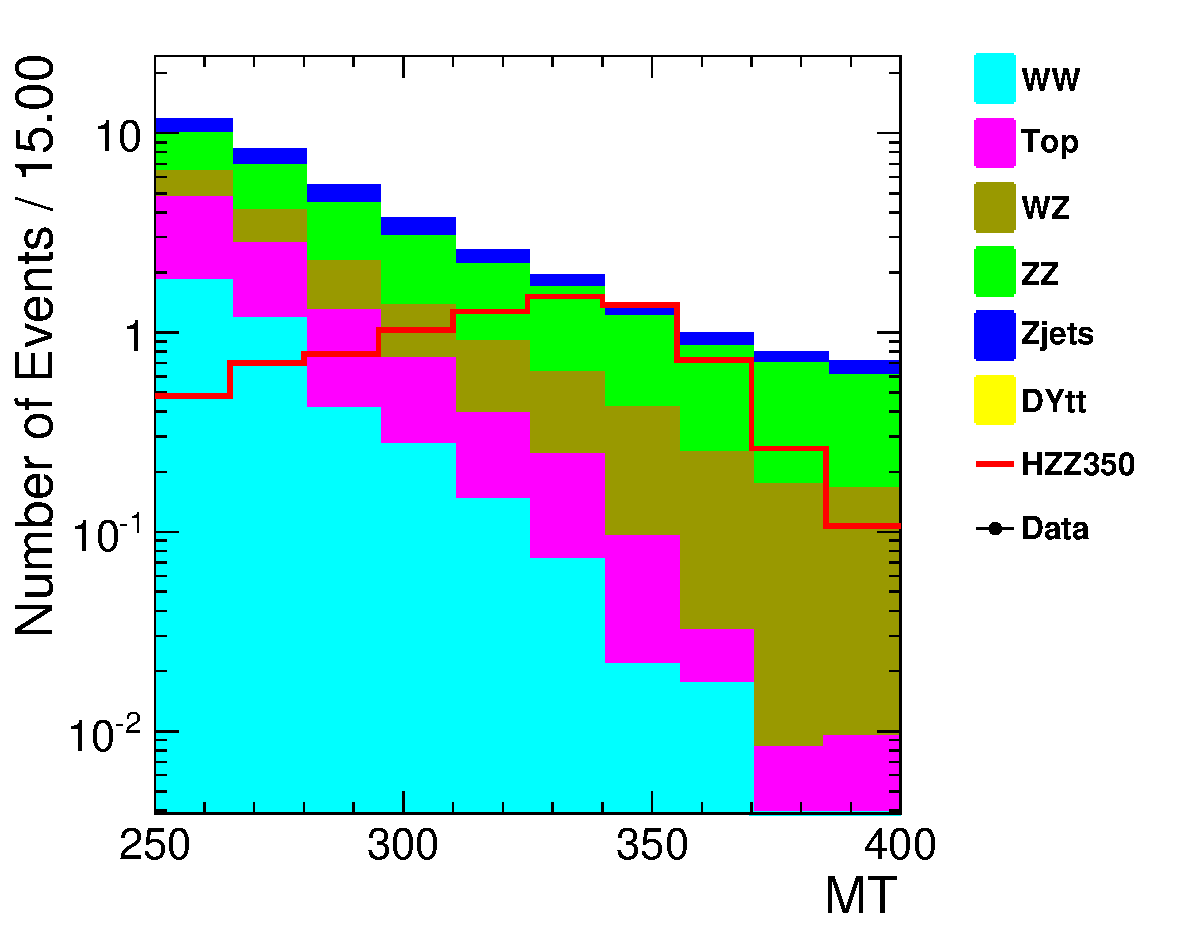
\includegraphics[width=0.4\textwidth,angle=0]{figures/MT_mH350_mm_stack_log.pdf}} \\ 
   \caption{The $M_T$ distribution for Higgs signal and background events 
for \mHi=350 $\GeVcc$ in ee (a) and $\mu\mu$ final state (b) after the higgs dependent selections. 
The distributions are normalized to \intlumi with the background scaled by the data-to-mc ratios derived from data.}
   \label{fig:histo_mt_350_5fb}
\end{center}
\end{figure}

\begin{figure}[!ht]
\begin{center}
   \subfigure[]{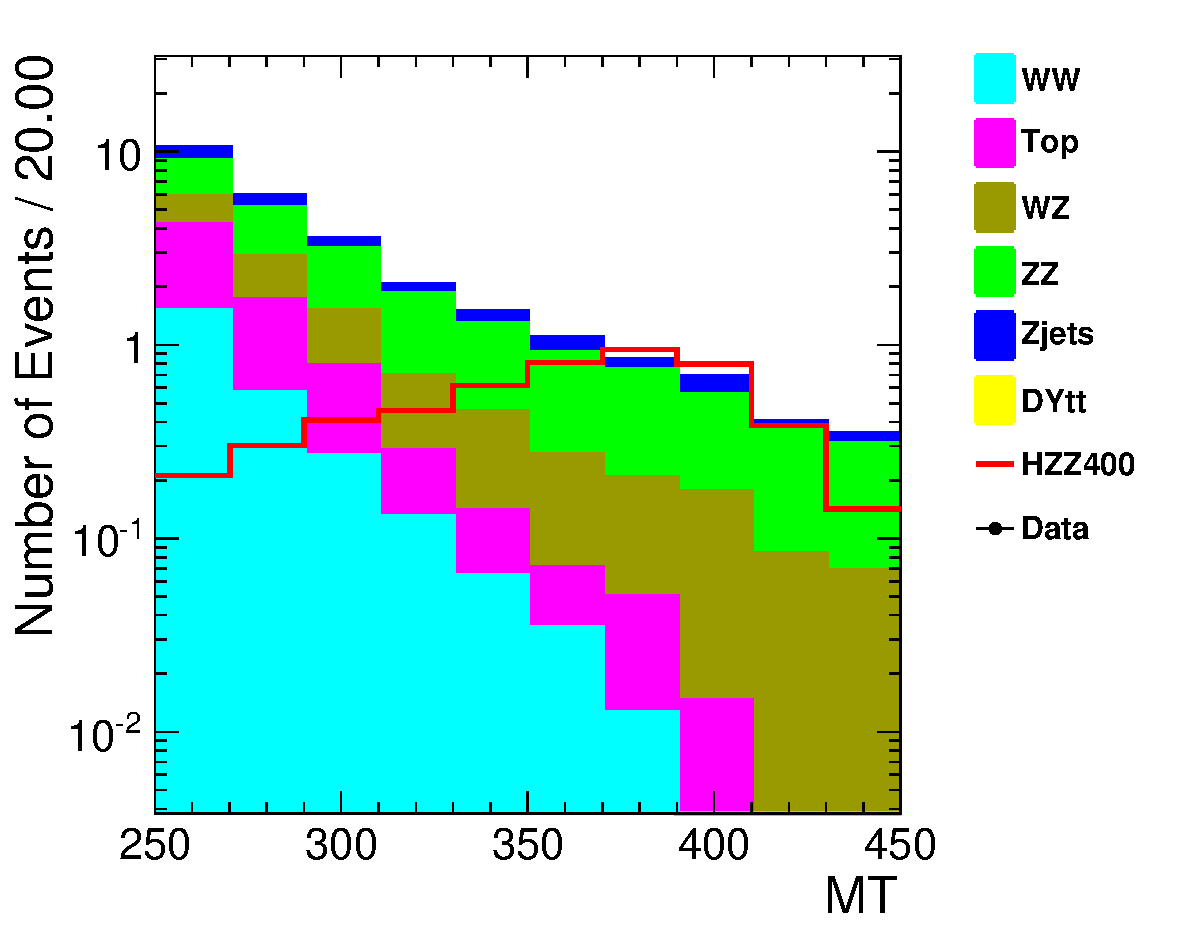
\includegraphics[width=0.4\textwidth,angle=0]{figures/MT_mH400_ee_stack_log.pdf}} 
   \subfigure[]{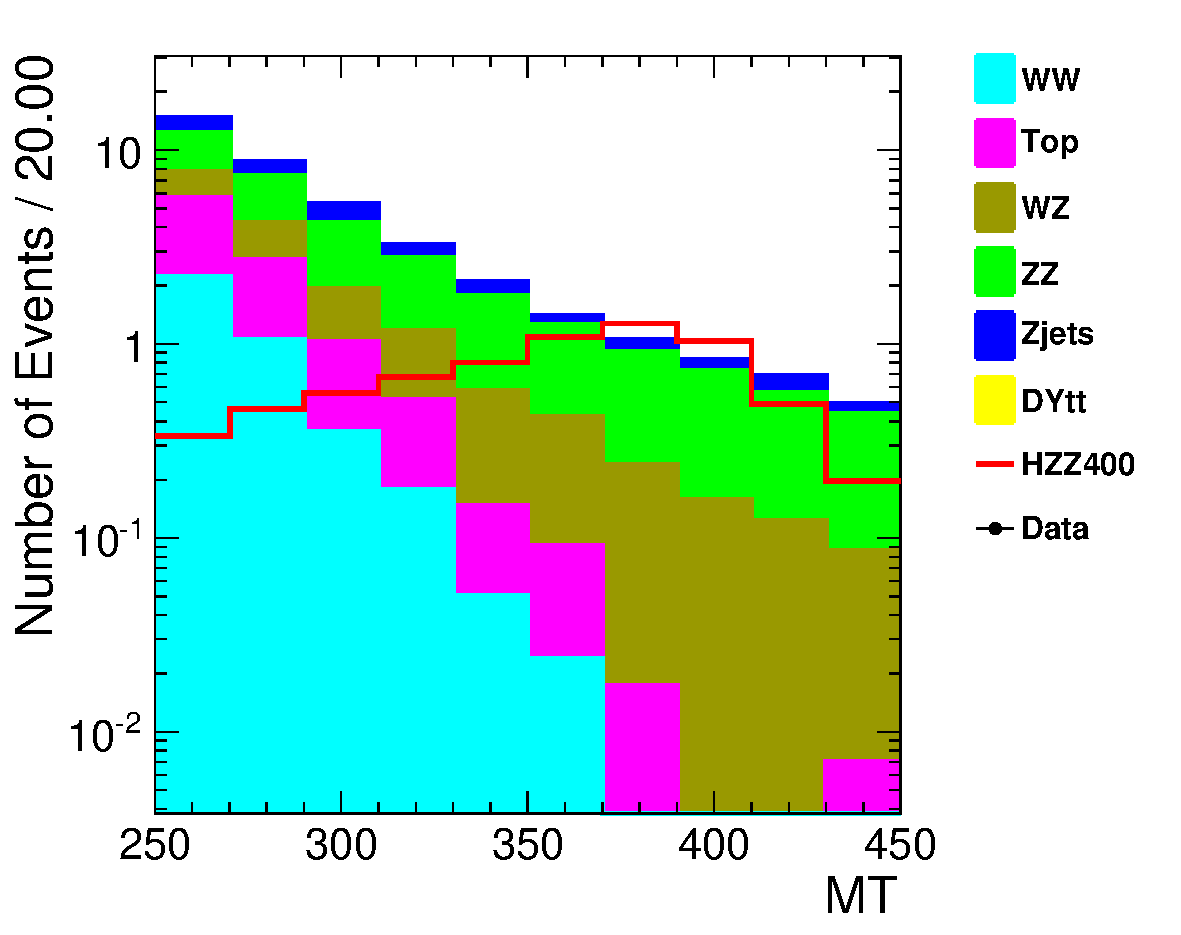
\includegraphics[width=0.4\textwidth,angle=0]{figures/MT_mH400_mm_stack_log.pdf}} \\ 
   \caption{The $M_T$ distribution for Higgs signal and background events 
for \mHi=400 $\GeVcc$ in ee (a) and $\mu\mu$ final state (b) after the higgs dependent selections. 
The distributions are normalized to \intlumi with the background scaled by the data-to-mc ratios derived from data.}
   \label{fig:histo_mt_400_5fb}
\end{center}
\end{figure}


\begin{figure}[!ht]
\begin{center}
   \subfigure[]{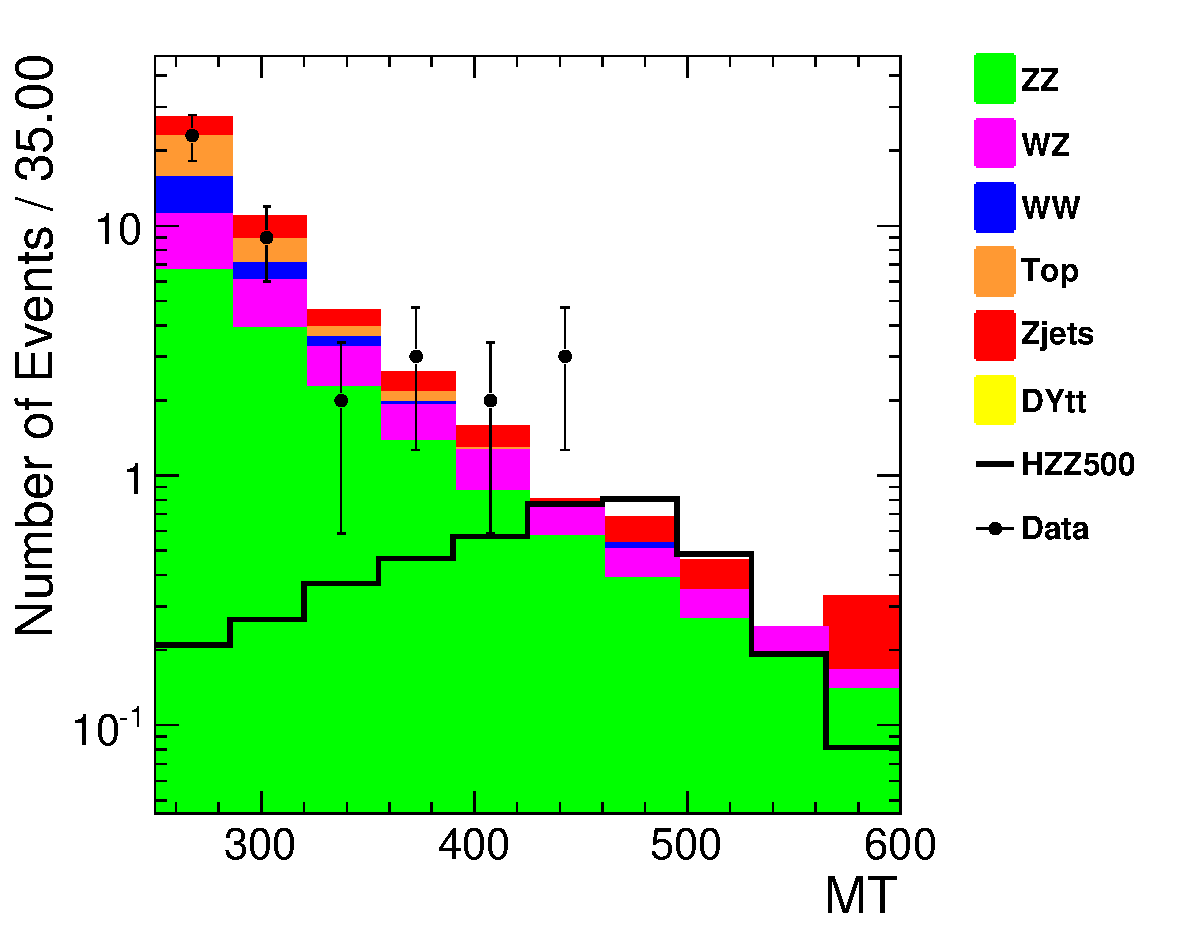
\includegraphics[width=0.4\textwidth,angle=0]{figures/MT_mH500_ee_stack_log.pdf}} 
   \subfigure[]{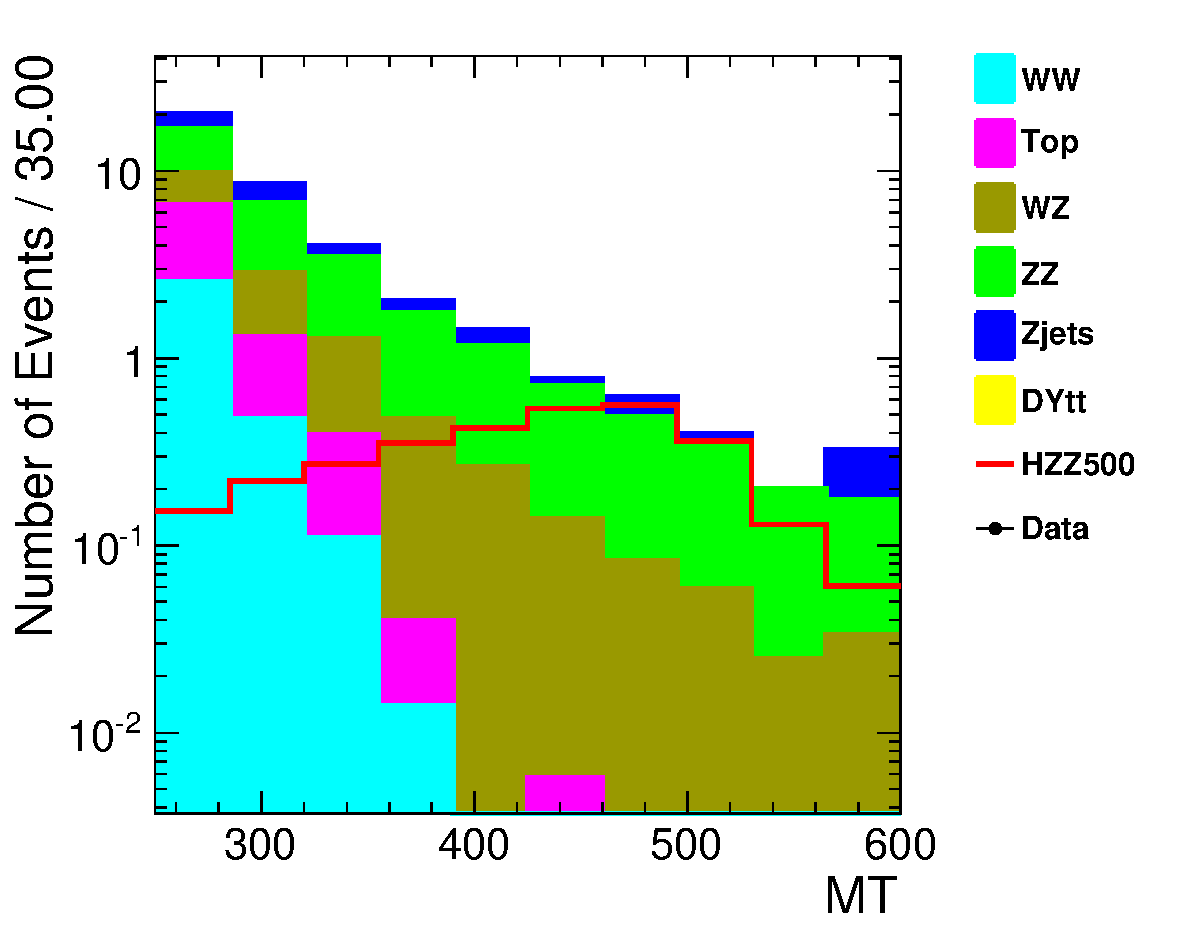
\includegraphics[width=0.4\textwidth,angle=0]{figures/MT_mH500_mm_stack_log.pdf}} \\ 
   \caption{The $M_T$ distribution for Higgs signal and background events 
for \mHi=500 $\GeVcc$ in ee (a) and $\mu\mu$ final state (b) after the higgs dependent selections. 
The distributions are normalized to \intlumi with the background scaled by the data-to-mc ratios derived from data.}
   \label{fig:histo_mt_500_5fb}
\end{center}
\end{figure}

\begin{figure}[!ht]
\begin{center}
   \subfigure[]{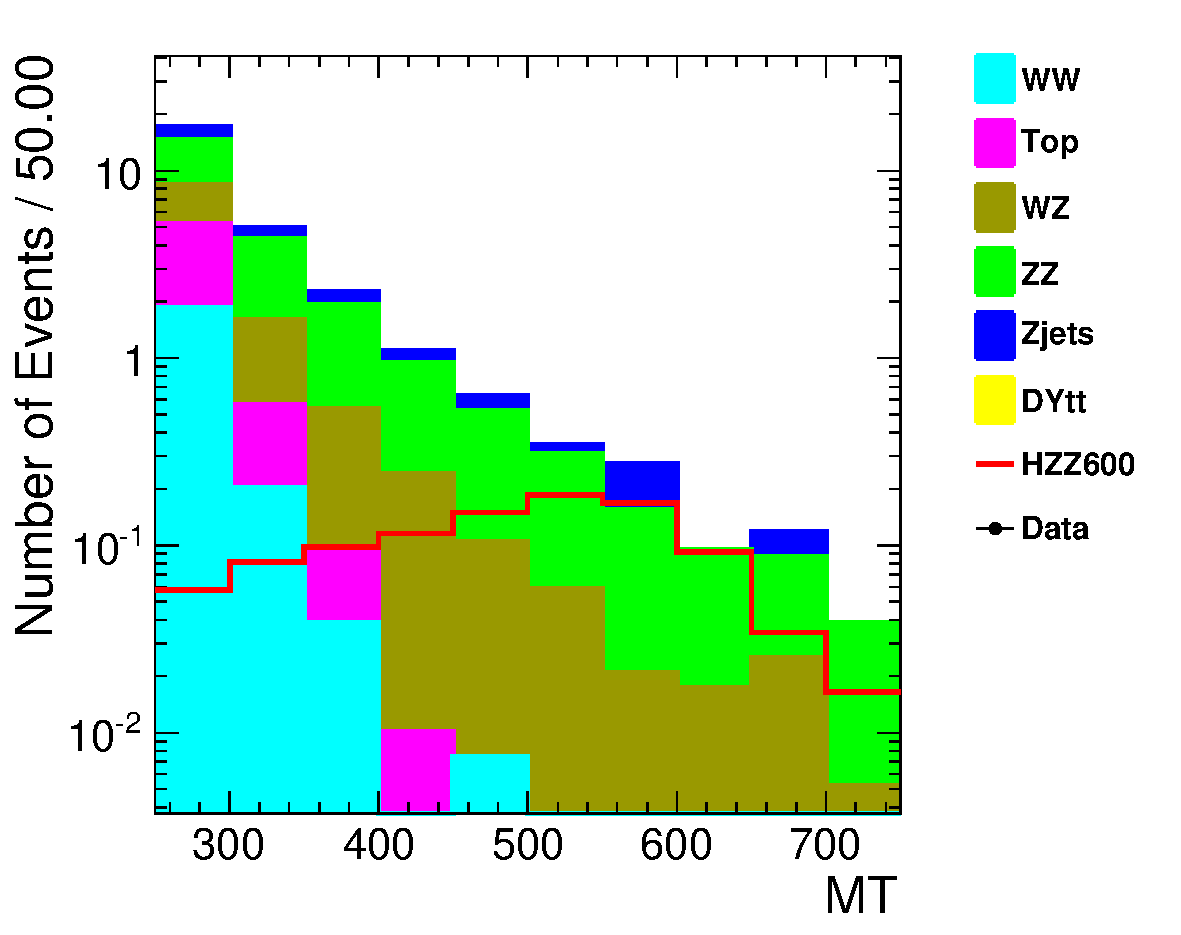
\includegraphics[width=0.4\textwidth,angle=0]{figures/MT_mH600_ee_stack_log.pdf}} 
   \subfigure[]{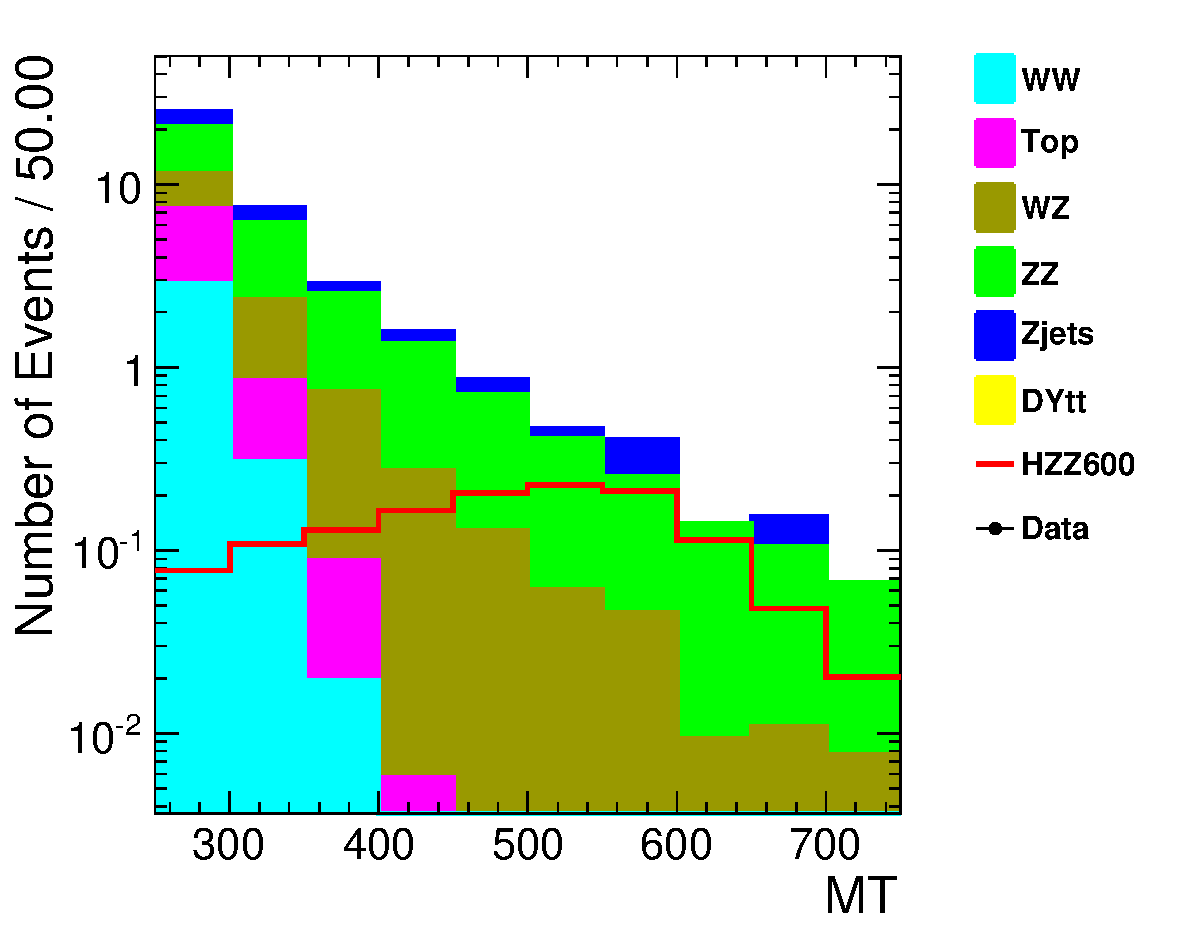
\includegraphics[width=0.4\textwidth,angle=0]{figures/MT_mH600_mm_stack_log.pdf}} \\ 
   \caption{The $M_T$ distribution for Higgs signal and background events 
for \mHi=600 $\GeVcc$ in ee (a) and $\mu\mu$ final state (b) after the higgs dependent selections. 
The distributions are normalized to \intlumi with the background scaled by the data-to-mc ratios derived from data.}
   \label{fig:histo_mt_600_5fb}
\end{center}
\end{figure}
%%%%%%%%%%%%%%%%%%%%%%

%%%%%%%%%%%%%%%%%%%%%%%%%%%%%
\begin{table}[!ht]
\begin{center}
{\normalsize
\begin{tabular}{|l|c|ccccc|}
\hline
      &  Analysis    & adding          &  adding      &  adding      & adding      & adding \\
mH  &  without     & template        &  $H\to ZZ$   &  Top/WW             & WZ          & ZZ \\
      &  shape syst. & stat. uncert.   &  QCD effect &  shape syst. & shape syst. & shape syst. \\
\hline
250 & 1.40 & 1.40 & 1.40 & 1.48 & 1.48 & 1.48 \\   
300 & 0.92 & 0.92 & 0.92 & 0.92 & 0.93 & 0.93 \\ 
350 & 0.62 & 0.62 & 0.62 & 0.63 & 0.63 & 0.63 \\
400 & 0.63 & 0.63 & 0.63 & 0.63 & 0.63 & 0.63 \\
500 & 1.06 & 1.06 & 1.06 & 1.06 & 1.08 & 1.08 \\
600 & 2.20 & 2.21 & 2.21 & 2.20 & 2.23 & 2.23 \\
\hline
\end{tabular}
}
\caption{Comparison of the median expected cross section ratio limits as a function 
of the Higgs mass between shape analysis without and with accouting for the 
shape variation systematics. The results on the various sources are added sequentially 
to study the impact of each source. } %Note that the statistical precision on the limits 
%here are around 1\%. }
\label{tab:mva_mtshape_detail}
\end{center}
\end{table}
%%%%%%%%%%%%%%%%%%%%%%%%%%%%%

%%%%%%%%%%%%%%%%%%%%%%%%%%%%%
\begin{figure}[!htbp]
\begin{center}
   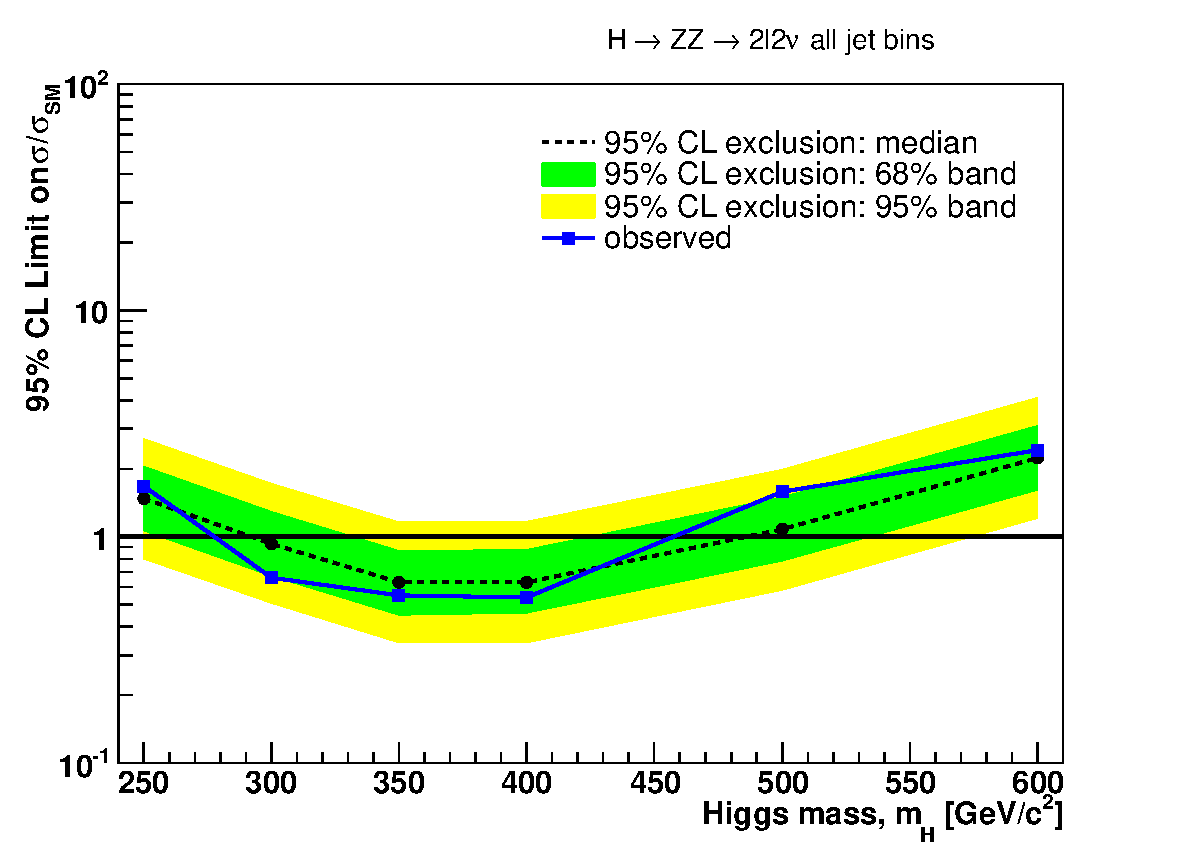
\includegraphics[width=0.8\textwidth]{figures/limits_mtshape_5fb.pdf}
   \caption{ The expected upper limits at 95\% C.L. for \intlumi\ of data for the shape based
    analyses. The $M_T$ shape analysis includes all the shape systematics. }
   \label{fig:limits_5fb}
\end{center}
\end{figure}
%%%%%%%%%%%%%%%%%%%%%%%%%%%%%
